% Für Bindekorrektur als optionales Argument "BCORfaktormitmaßeinheit", dann
% sieht auch Option "twoside" vernünftig aus
% Näheres zu "scrartcl" bzw. "scrreprt" und "scrbook" siehe KOMA-Skript Doku
\documentclass[12pt,a4paper,titlepage,headinclude,bibtotoc]{scrartcl}


%---- Allgemeine Layout Einstellungen ------------------------------------------

% Für Kopf und Fußzeilen, siehe auch KOMA-Skript Doku
\usepackage[komastyle]{scrpage2}
\pagestyle{scrheadings}
\automark[section]{chapter}
\setheadsepline{0.5pt}[\color{black}]

%keine Einrückung
\parindent0pt

%Einstellungen für Figuren- und Tabellenbeschriftungen
\setkomafont{captionlabel}{\sffamily\bfseries}
\setcapindent{0em}

\usepackage{caption}

%---- Weitere Pakete -----------------------------------------------------------
% Die Pakete sind alle in der TeX Live Distribution enthalten. Wichtige Adressen
% www.ctan.org, www.dante.de

% Sprachunterstützung
\usepackage[ngerman]{babel}

% Benutzung von Umlauten direkt im Text
% entweder "latin1" oder "utf8"
\usepackage[utf8]{inputenc}

% Pakete mit Mathesymbolen und zur Beseitigung von Schwächen der Mathe-Umgebung
\usepackage{latexsym,exscale,amssymb,amsmath}

% Weitere Symbole
\usepackage[nointegrals]{wasysym}
\usepackage{eurosym}

% Anderes Literaturverzeichnisformat
%\usepackage[square,sort&compress]{natbib}

% Für Farbe
\usepackage{color}

% Zur Graphikausgabe
%Beipiel: \includegraphics[width=\textwidth]{grafik.png}
\usepackage{graphicx}

% Text umfließt Graphiken und Tabellen
% Beispiel:
% \begin{wrapfigure}[Zeilenanzahl]{"l" oder "r"}{breite}
%   \centering
%   \includegraphics[width=...]{grafik}
%   \caption{Beschriftung} 
%   \label{fig:grafik}
% \end{wrapfigure}
\usepackage{wrapfig}

% Mehrere Abbildungen nebeneinander
% Beispiel:
% \begin{figure}[htb]
%   \centering
%   \subfigure[Beschriftung 1\label{fig:label1}]
%   {\includegraphics[width=0.49\textwidth]{grafik1}}
%   \hfill
%   \subfigure[Beschriftung 2\label{fig:label2}]
%   {\includegraphics[width=0.49\textwidth]{grafik2}}
%   \caption{Beschriftung allgemein}
%   \label{fig:label-gesamt}
% \end{figure}
\usepackage{subfigure}
\usepackage{adjustbox}

% Caption neben Abbildung
% Beispiel:
% \sidecaptionvpos{figure}{"c" oder "t" oder "b"}
% \begin{SCfigure}[rel. Breite (normalerweise = 1)][hbt]
%   \centering
%   \includegraphics[width=0.5\textwidth]{grafik.png}
%   \caption{Beschreibung}
%   \label{fig:}
% \end{SCfigure}
\usepackage{sidecap}

% Befehl für "Entspricht"-Zeichen
\newcommand{\corresponds}{\ensuremath{\mathrel{\widehat{=}}}}

%Für chemische Formeln (von www.dante.de)
%% Anpassung an LaTeX(2e) von Bernd Raichle
\makeatletter
\DeclareRobustCommand{\chemical}[1]{%
  {\(\m@th
   \edef\resetfontdimens{\noexpand\)%
       \fontdimen16\textfont2=\the\fontdimen16\textfont2
       \fontdimen17\textfont2=\the\fontdimen17\textfont2\relax}%
   \fontdimen16\textfont2=2.7pt \fontdimen17\textfont2=2.7pt
   \mathrm{#1}%
   \resetfontdimens}}
\makeatother

%Si Einheiten
\usepackage{siunitx}

%c++ Code einbinden
\usepackage{listings}
\lstset{numbers=left, numberstyle=\tiny, numbersep=5pt}

%Differential
\newcommand{\dif}{\ensuremath{\mathrm{d}}}

%Boxen,etc.
\usepackage{fancybox}
\usepackage{empheq}

%Fußnoten auf gleiche Seite
\interfootnotelinepenalty=1000

%Dateien aus Unterverzeichnissen
\usepackage{import}

%Bibliography \bibliography{literatur} und \cite{gerthsen}
%\usepackage{cite}
\usepackage{babelbib}
\selectbiblanguage{ngerman}

\begin{document}

\begin{titlepage}
\centering
\textsc{\Large Anfängerpraktikum der Fakultät für
  Physik,\\[1.5ex] Universität Göttingen}

\vspace*{4.2cm}

\rule{\textwidth}{1pt}\\[0.5cm]
{\huge \bfseries
  Fresnelsche Formeln und\\[1.5ex]
  und Polarisation}\\[0.5cm]
\rule{\textwidth}{1pt}

\vspace*{3.0cm}

\begin{Large}
\begin{tabular}{ll}
Praktikant:
 	&  Felix Kurtz\\
Versuchspartner:
 	&  Michael Lohmann\\

E-Mail: 
	&  felix.kurtz@stud.uni-goettingen.de\\
	
 Betreuer: & Phillip Bastian\\
 Versuchsdatum: &  06.03.2015\\
\end{tabular}
\end{Large}

\vspace*{1.8cm}

\begin{Large}
\fbox{
  \begin{minipage}[t][2.5cm][t]{6cm} 
    Eingegangen am:
  \end{minipage}
}
\end{Large}

\end{titlepage}

\tableofcontents

\newpage

\section{Einleitung}
\label{sec:einleitung}
In diesem Versuch steht die elektromagnetische Natur des Lichts im Vordergrund.
So kann man Licht \emph{polarisieren}.
Dieses Phänomen ist zum Beispiel wichtig für 3D-Filme.
Außerdem soll der \emph{Brewster-Winkel} vermessen werden.
Unter diesem Winkel ist der reflektierte Anteil minimal.
Dies folgt aus den \emph{Fresnelschen Formeln}, die zum Beispiel angeben, wie groß der reflektierte Anteil ist.\\
Bei der Messung spielt die \emph{Doppelbrechung} eine große Rolle.

\section{Theorie}
\label{sec:theorie}
\subsection{Polarisation}
Licht ist eine elektromagnetische Transversalwelle.
Die Ausbreitungsrichtung, das elektrische E-Feld sowie das magnetische B-Feld stehen dabei jeweils senkrecht aufeinander.
Polarisiert man diese Welle \emph{linear}, so schwingt das elektrische Feld immer in einer bestimmten Ebene.
Diese ändert sich zeitlich nicht.
Mehr dazu wird in \cite[S.233ff.]{saleh-teich} erläutert.

\subsection{Fresnelsche Formeln}
\begin{figure}[!h]
	\centering	
	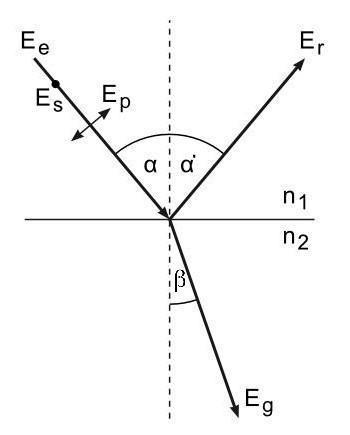
\includegraphics[scale=0.35]{Reflexion_Brechung.jpg}
	\caption{Reflexion und Brechung an einer Grenzschicht nach \cite[Datum: 23.03.2015]{LP20}.}	
	\label{fig:Reflexion_Brechung}
\end{figure}

Trifft Licht mit der Amplitude $E_e$ auf eine Grenzfläche wie in Abbildung \ref{fig:Reflexion_Brechung}, wird ein Teil $E_r$ davon reflektiert, der Andere, $E_g$, transmittiert.
Dabei gelten nun zunächst die Winkelbeziehungen \glqq Einfallswinkel gleich Ausfallswinkel\grqq , also $\alpha=\alpha'$, sowie das Snelliussche Brechungsgesetz \cite[S.6]{saleh-teich}
\begin{align}
	n_1\sin\alpha=n_2\sin\beta\,,
	\label{eq:snellius}
\end{align}
mit den Brechungsindizes $n_1$ des ersten Mediums und $n_2$ des zweiten.
Das E-Feld lässt sich parallel und senkrecht zur Einfallsebene zerlegen, die durch den einfallenden Strahl und dem Lot gebildet wird.
Die aus den Maxwellschen Gleichungen abgeleitete Stetigkeit der Tangentialkomponenten des E-Feldes bei einem Übergang sowie die Energieerhaltung führen zu den \emph{Fresnel Formeln}, die die Amplitudenverhältnisse bei solch einem Übergang beschreiben.
So wird das Verhältnis $r:=\frac{E_r}{E_e}$ als Reflexionskoeffizient bezeichnet.
Für den senkrechten sowie parallelen Fall folgt
\begin{align}
	r_s&=-\frac{\sin(\alpha-\beta)}{\sin(\alpha+\beta)}\qquad \text{und}
	\label{eq:r_s}\\
	r_p&=\frac{\tan(\alpha-\beta)}{\tan(\alpha+\beta)}\,.
	\label{eq:r_p}
\end{align}
Dabei gilt das Snellius'sche Brechungsgesetz \eqref{eq:snellius}.
Die genaue Herleitung kann in \cite[S.237ff.]{demtroeder2} nachgelsen werden.\\
Das Quadrat des Reflexionskoeffizienten $R:=r^2$ gibt das Intensitätsverhältnis von reflektiertem zu einfallendem Strahl an, da die Intensität $I$ proportional zum Quadrat der Amplitude $E$ ist.
In Abbildung \ref{fig:fresnelkoeff} ist $R$ in Abhängigkeit vom Einfallswinkel $\alpha$ für beide Fälle aufgetragen.
Bei $\alpha=90^\circ$ wird unabhängig von der Polarisationsrichtung $100\%$ reflektiert.
Über die Energieerhaltung kann der relative Transmissionsanteil $T$ der Intensität berechnet werden (vgl. \cite[S.239]{demtroeder2}):
\begin{align}
	T=1-R\,.
\end{align}

\begin{figure}[!h]
	\centering
	% GNUPLOT: LaTeX picture with Postscript
\begingroup
  \makeatletter
  \providecommand\color[2][]{%
    \GenericError{(gnuplot) \space\space\space\@spaces}{%
      Package color not loaded in conjunction with
      terminal option `colourtext'%
    }{See the gnuplot documentation for explanation.%
    }{Either use 'blacktext' in gnuplot or load the package
      color.sty in LaTeX.}%
    \renewcommand\color[2][]{}%
  }%
  \providecommand\includegraphics[2][]{%
    \GenericError{(gnuplot) \space\space\space\@spaces}{%
      Package graphicx or graphics not loaded%
    }{See the gnuplot documentation for explanation.%
    }{The gnuplot epslatex terminal needs graphicx.sty or graphics.sty.}%
    \renewcommand\includegraphics[2][]{}%
  }%
  \providecommand\rotatebox[2]{#2}%
  \@ifundefined{ifGPcolor}{%
    \newif\ifGPcolor
    \GPcolortrue
  }{}%
  \@ifundefined{ifGPblacktext}{%
    \newif\ifGPblacktext
    \GPblacktexttrue
  }{}%
  % define a \g@addto@macro without @ in the name:
  \let\gplgaddtomacro\g@addto@macro
  % define empty templates for all commands taking text:
  \gdef\gplbacktext{}%
  \gdef\gplfronttext{}%
  \makeatother
  \ifGPblacktext
    % no textcolor at all
    \def\colorrgb#1{}%
    \def\colorgray#1{}%
  \else
    % gray or color?
    \ifGPcolor
      \def\colorrgb#1{\color[rgb]{#1}}%
      \def\colorgray#1{\color[gray]{#1}}%
      \expandafter\def\csname LTw\endcsname{\color{white}}%
      \expandafter\def\csname LTb\endcsname{\color{black}}%
      \expandafter\def\csname LTa\endcsname{\color{black}}%
      \expandafter\def\csname LT0\endcsname{\color[rgb]{1,0,0}}%
      \expandafter\def\csname LT1\endcsname{\color[rgb]{0,1,0}}%
      \expandafter\def\csname LT2\endcsname{\color[rgb]{0,0,1}}%
      \expandafter\def\csname LT3\endcsname{\color[rgb]{1,0,1}}%
      \expandafter\def\csname LT4\endcsname{\color[rgb]{0,1,1}}%
      \expandafter\def\csname LT5\endcsname{\color[rgb]{1,1,0}}%
      \expandafter\def\csname LT6\endcsname{\color[rgb]{0,0,0}}%
      \expandafter\def\csname LT7\endcsname{\color[rgb]{1,0.3,0}}%
      \expandafter\def\csname LT8\endcsname{\color[rgb]{0.5,0.5,0.5}}%
    \else
      % gray
      \def\colorrgb#1{\color{black}}%
      \def\colorgray#1{\color[gray]{#1}}%
      \expandafter\def\csname LTw\endcsname{\color{white}}%
      \expandafter\def\csname LTb\endcsname{\color{black}}%
      \expandafter\def\csname LTa\endcsname{\color{black}}%
      \expandafter\def\csname LT0\endcsname{\color{black}}%
      \expandafter\def\csname LT1\endcsname{\color{black}}%
      \expandafter\def\csname LT2\endcsname{\color{black}}%
      \expandafter\def\csname LT3\endcsname{\color{black}}%
      \expandafter\def\csname LT4\endcsname{\color{black}}%
      \expandafter\def\csname LT5\endcsname{\color{black}}%
      \expandafter\def\csname LT6\endcsname{\color{black}}%
      \expandafter\def\csname LT7\endcsname{\color{black}}%
      \expandafter\def\csname LT8\endcsname{\color{black}}%
    \fi
  \fi
  \setlength{\unitlength}{0.0500bp}%
  \begin{picture}(7200.00,5040.00)%
    \gplgaddtomacro\gplbacktext{%
      \csname LTb\endcsname%
      \put(946,704){\makebox(0,0)[r]{\strut{} 0}}%
      \put(946,1111){\makebox(0,0)[r]{\strut{} 0.1}}%
      \put(946,1518){\makebox(0,0)[r]{\strut{} 0.2}}%
      \put(946,1925){\makebox(0,0)[r]{\strut{} 0.3}}%
      \put(946,2332){\makebox(0,0)[r]{\strut{} 0.4}}%
      \put(946,2740){\makebox(0,0)[r]{\strut{} 0.5}}%
      \put(946,3147){\makebox(0,0)[r]{\strut{} 0.6}}%
      \put(946,3554){\makebox(0,0)[r]{\strut{} 0.7}}%
      \put(946,3961){\makebox(0,0)[r]{\strut{} 0.8}}%
      \put(946,4368){\makebox(0,0)[r]{\strut{} 0.9}}%
      \put(946,4775){\makebox(0,0)[r]{\strut{} 1}}%
      \put(1078,484){\makebox(0,0){\strut{} 0}}%
      \put(1714,484){\makebox(0,0){\strut{} 10}}%
      \put(2350,484){\makebox(0,0){\strut{} 20}}%
      \put(2986,484){\makebox(0,0){\strut{} 30}}%
      \put(3622,484){\makebox(0,0){\strut{} 40}}%
      \put(4259,484){\makebox(0,0){\strut{} 50}}%
      \put(4895,484){\makebox(0,0){\strut{} 60}}%
      \put(5531,484){\makebox(0,0){\strut{} 70}}%
      \put(6167,484){\makebox(0,0){\strut{} 80}}%
      \put(6803,484){\makebox(0,0){\strut{} 90}}%
      \put(176,2739){\rotatebox{-270}{\makebox(0,0){\strut{}Reflexionskoeffizient $R$}}}%
      \put(3940,154){\makebox(0,0){\strut{}Einfallswinkel $\alpha$ [$^\circ$]}}%
    }%
    \gplgaddtomacro\gplfronttext{%
      \csname LTb\endcsname%
      \put(5816,4602){\makebox(0,0)[r]{\strut{}senkrecht}}%
      \csname LTb\endcsname%
      \put(5816,4382){\makebox(0,0)[r]{\strut{}parallel}}%
    }%
    \gplbacktext
    \put(0,0){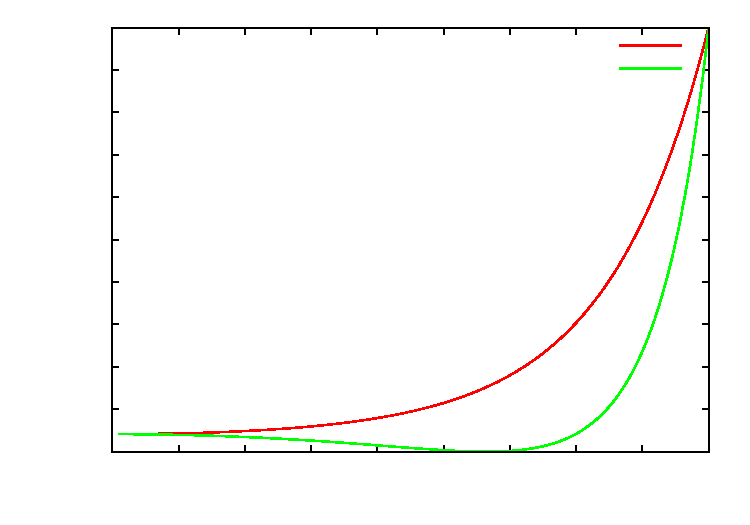
\includegraphics{fresnelkoeff}}%
    \gplfronttext
  \end{picture}%
\endgroup

	\caption{Fresnelkoeffizienten für $n_1=1$ und $n_2=1.51$.}
	\label{fig:fresnelkoeff}
\end{figure}

\subsection{Brewster-Winkel}
Nach \eqref{eq:r_p} verschwindet der Reflexionskoeffizient $r_p$, wenn $\alpha+\beta=90^\circ$, denn dann ist $\tan(\alpha+\beta)=\infty$.
Setzt man nun die Beziehung \eqref{eq:snellius} ein, kann man diesen Einfallswinkel $\alpha_B$, den sogenannten \emph{Brewster-Winkel} (vgl. dazu \cite[S.240]{demtroeder2}), über
\begin{align}
	\tan\alpha_\text{B}=\frac{n_2}{n_1}
	\label{eq:brewster}
\end{align}
berechnen, bei dem keine Reflexion von parallelem Licht auftritt.
Dies ist auch in Abbildung \ref{fig:fresnelkoeff} gut zu erkennen ($\alpha_B=56.49^\circ$ bei $n=\frac{n_2}{n_1}=1.51$).

\subsection{Doppelbrechung}
Anisotrope Kristalle besitzen eine ausgezeichnete Achse, die sogenannte optische Achse.
Der Brechungsindex in Richtung dieser Achse ist ein anderer als der senkrecht dazu.
Dadurch teilt sich der Strahl in einen ordentlichen, der senkrecht zur optischen Achse polarisiert ist und nach dem Snelliusschen Brechungsgesetz gebrochen wird,  und einen außerordentlichen Strahl auf, der in Richtung der optischen Achse polarisiert ist.
Letzterer wird zum Beispiel auch bei senkrechtem Einfall gebrochen, gehorcht Snellius also nicht.
Näheres findet man in \cite[S.264ff.]{saleh-teich}.\\
Ein Anwendungsbeispiel der Doppelbrechung ist das Nicol-Prisma (vgl. \cite[S.255]{demtroeder2}), welches in Abbildung \ref{fig:nicol} schematisch dargestellt ist.
Während der ordentliche Strahl gebrochen wird und somit nach einer Totalreflexion auf eine absorbierende Schicht trifft, kann der außerordentliche Strahl das Prisma ungehindert passieren.
So gelangt nur das in Richtung der optischen Achse polarisierte Licht hindurch.

\begin{figure}[!h]
	\centering
	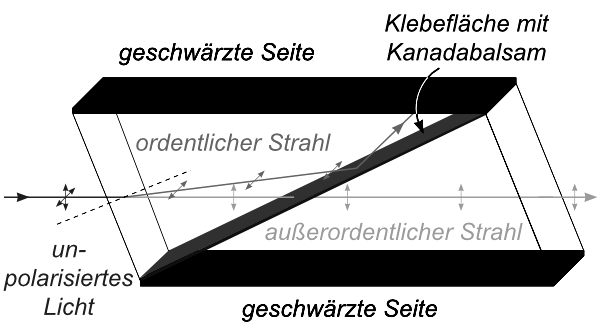
\includegraphics[scale=0.7]{nicol.png}
	\caption{Strahlengang im Nicolschen Prisma. \cite[Datum: 23.03.2015]{LP20}}
	\label{fig:nicol}
\end{figure}

\section{Durchführung}
\label{sec:durchfuehrung}
In Abbildung \ref{fig:aufbau} ist der Aufbau schematisch dargestellt.
Das Licht stammt von einer Quecksilberdampflampe, deren grüne Linie nach einer Linse und einer Blende durch einen Filter durchgelassen wird.
Danach trifft der Strahl auf einen drehbaren Polarisator, ist also linear polarisiert, wenn er auf das Prisma trifft, welches sich auf einem Drehteller befindet.
Lenkt man den Schwenkarm um einen Winkel $\Phi$ aus, so dreht der Teller sich um den halben Winkel, sodass man den reflektierten Strahl immer durch das Okular sehen kann, falls das Prisma richtig positioniert ist.
Auf dem Schwenkarm kann noch der Analysator befestigt werden, also ein drehbares Nicol-Prisma.\\ 

Zuerst muss der Strahlengang justiert werden.
Dazu wird das evtl. noch im Strahlengang stehende Glasprisma entfernt und Polarisator und Analysator durchlässig gedreht.
Mit den Linsen bildet man das grüne Lichtbündel scharf auf das Okular ab.
Nun wird die Polarisationsrichtung justiert.
Dabei wird das kleine Nicolsche Prisma auf den Drehteller gestellt.
Die optische Achse des Prismas zeigt nach oben.
Man entfernt den Analysator und dreht den Polarisator, so dass im Okular kein Strahl mehr zu sehen ist.
Dann steht der Polarisator parallel zur Einfallsebene.
Jetzt wird dieser um $45^\circ$ gedreht.
Die eine Hälfte ist nun parallel, die andere senkrecht zur Einfallsebene polarisiert.
Danach wird das Glasprisma auf dem Drehteller justiert.
Meist sind Markierungen schon vorhanden.
Man prüft, ob man den Strahl durch das Okular beobachten kann, wenn der Schwenkarm nicht sowie um $90^\circ$ ausgelenkt ist.
Sollte dies nicht der Fall sein, muss nachjustiert werden.\\

Nun kann man den Reflexionskoeffizienten messen.
Dazu wird der Analysator wieder in den Strahlengang gestellt.
In $5^\circ$-Schritten wird der Schwenkarm nun von $0^\circ$ bis $90^\circ$ ausgelenkt.
Dabei dreht man den Analysator immer so, dass Dunkelheit im Okular herrscht.
Der so eingestellte Winkel wird an der Winkelskala abgelesen und notiert.\\

Zuletzt wird der Brewster-Winkel gemessen.
Dazu muss der Polarisator wieder um $45^\circ$ zurück gedreht werden, damit das Licht parallel polarisiert ist.
Der Analysator wird entfernt.
Man bestimmt mehrmals den Auslenkwinkel des Schwenkarms, bei dem ein Intensitätsminimum des reflektierten Strahls durch das Okular beobachtet wird.

\begin{figure}[!h]
	\centering
	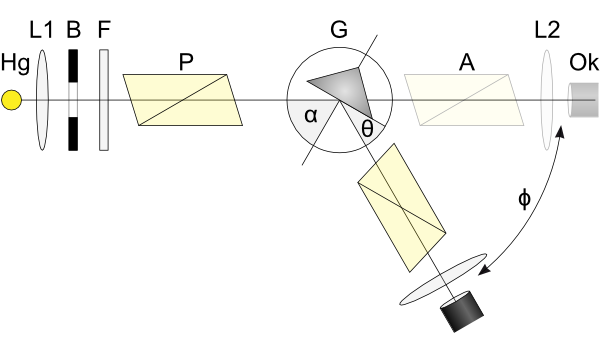
\includegraphics[scale=0.5]{aufbau_schema.png}
	\caption{Versuchsaufbau schematisch. \cite[Datum: 23.03.2015]{LP20}}
	\label{fig:aufbau}
\end{figure}

\section{Auswertung}
\label{sec:auswertung}
Die gemessene Auslenkung des Schwenkarms $\Phi$ muss zunächst umgerechnet werden, um den Winkel $\alpha$ zum Lot der Prismaoberfläche zu erhalten (vgl. Abb.\ref{fig:aufbau}):\\
\begin{align}
	\alpha=90^\circ-\frac{1}{2}\Phi\,.
\end{align}
Außerdem ist $n_1=1$ (Luft) und der Brechungsindex für das Prismenglas sollte bei $n := n_2=1.510 \pm 0.005$ liegen \cite[S.181]{prakti}.
Er wird durch die beiden Messungen und verschiedene Methoden bestimmt.

\subsection{Drehung der Schwingungsebene}

\begin{figure}[!htb]
	\centering
	% GNUPLOT: LaTeX picture with Postscript
\begingroup
  \makeatletter
  \providecommand\color[2][]{%
    \GenericError{(gnuplot) \space\space\space\@spaces}{%
      Package color not loaded in conjunction with
      terminal option `colourtext'%
    }{See the gnuplot documentation for explanation.%
    }{Either use 'blacktext' in gnuplot or load the package
      color.sty in LaTeX.}%
    \renewcommand\color[2][]{}%
  }%
  \providecommand\includegraphics[2][]{%
    \GenericError{(gnuplot) \space\space\space\@spaces}{%
      Package graphicx or graphics not loaded%
    }{See the gnuplot documentation for explanation.%
    }{The gnuplot epslatex terminal needs graphicx.sty or graphics.sty.}%
    \renewcommand\includegraphics[2][]{}%
  }%
  \providecommand\rotatebox[2]{#2}%
  \@ifundefined{ifGPcolor}{%
    \newif\ifGPcolor
    \GPcolortrue
  }{}%
  \@ifundefined{ifGPblacktext}{%
    \newif\ifGPblacktext
    \GPblacktexttrue
  }{}%
  % define a \g@addto@macro without @ in the name:
  \let\gplgaddtomacro\g@addto@macro
  % define empty templates for all commands taking text:
  \gdef\gplbacktext{}%
  \gdef\gplfronttext{}%
  \makeatother
  \ifGPblacktext
    % no textcolor at all
    \def\colorrgb#1{}%
    \def\colorgray#1{}%
  \else
    % gray or color?
    \ifGPcolor
      \def\colorrgb#1{\color[rgb]{#1}}%
      \def\colorgray#1{\color[gray]{#1}}%
      \expandafter\def\csname LTw\endcsname{\color{white}}%
      \expandafter\def\csname LTb\endcsname{\color{black}}%
      \expandafter\def\csname LTa\endcsname{\color{black}}%
      \expandafter\def\csname LT0\endcsname{\color[rgb]{1,0,0}}%
      \expandafter\def\csname LT1\endcsname{\color[rgb]{0,1,0}}%
      \expandafter\def\csname LT2\endcsname{\color[rgb]{0,0,1}}%
      \expandafter\def\csname LT3\endcsname{\color[rgb]{1,0,1}}%
      \expandafter\def\csname LT4\endcsname{\color[rgb]{0,1,1}}%
      \expandafter\def\csname LT5\endcsname{\color[rgb]{1,1,0}}%
      \expandafter\def\csname LT6\endcsname{\color[rgb]{0,0,0}}%
      \expandafter\def\csname LT7\endcsname{\color[rgb]{1,0.3,0}}%
      \expandafter\def\csname LT8\endcsname{\color[rgb]{0.5,0.5,0.5}}%
    \else
      % gray
      \def\colorrgb#1{\color{black}}%
      \def\colorgray#1{\color[gray]{#1}}%
      \expandafter\def\csname LTw\endcsname{\color{white}}%
      \expandafter\def\csname LTb\endcsname{\color{black}}%
      \expandafter\def\csname LTa\endcsname{\color{black}}%
      \expandafter\def\csname LT0\endcsname{\color{black}}%
      \expandafter\def\csname LT1\endcsname{\color{black}}%
      \expandafter\def\csname LT2\endcsname{\color{black}}%
      \expandafter\def\csname LT3\endcsname{\color{black}}%
      \expandafter\def\csname LT4\endcsname{\color{black}}%
      \expandafter\def\csname LT5\endcsname{\color{black}}%
      \expandafter\def\csname LT6\endcsname{\color{black}}%
      \expandafter\def\csname LT7\endcsname{\color{black}}%
      \expandafter\def\csname LT8\endcsname{\color{black}}%
    \fi
  \fi
    \setlength{\unitlength}{0.0500bp}%
    \ifx\gptboxheight\undefined%
      \newlength{\gptboxheight}%
      \newlength{\gptboxwidth}%
      \newsavebox{\gptboxtext}%
    \fi%
    \setlength{\fboxrule}{0.5pt}%
    \setlength{\fboxsep}{1pt}%
\begin{picture}(7200.00,5040.00)%
    \gplgaddtomacro\gplbacktext{%
      \csname LTb\endcsname%
      \put(814,704){\makebox(0,0)[r]{\strut{}$-10$}}%
      \put(814,1213){\makebox(0,0)[r]{\strut{}$0$}}%
      \put(814,1722){\makebox(0,0)[r]{\strut{}$10$}}%
      \put(814,2231){\makebox(0,0)[r]{\strut{}$20$}}%
      \put(814,2740){\makebox(0,0)[r]{\strut{}$30$}}%
      \put(814,3248){\makebox(0,0)[r]{\strut{}$40$}}%
      \put(814,3757){\makebox(0,0)[r]{\strut{}$50$}}%
      \put(814,4266){\makebox(0,0)[r]{\strut{}$60$}}%
      \put(814,4775){\makebox(0,0)[r]{\strut{}$70$}}%
      \put(946,484){\makebox(0,0){\strut{}$45$}}%
      \put(1597,484){\makebox(0,0){\strut{}$50$}}%
      \put(2248,484){\makebox(0,0){\strut{}$55$}}%
      \put(2898,484){\makebox(0,0){\strut{}$60$}}%
      \put(3549,484){\makebox(0,0){\strut{}$65$}}%
      \put(4200,484){\makebox(0,0){\strut{}$70$}}%
      \put(4851,484){\makebox(0,0){\strut{}$75$}}%
      \put(5501,484){\makebox(0,0){\strut{}$80$}}%
      \put(6152,484){\makebox(0,0){\strut{}$85$}}%
      \put(6803,484){\makebox(0,0){\strut{}$90$}}%
    }%
    \gplgaddtomacro\gplfronttext{%
      \csname LTb\endcsname%
      \put(176,2739){\rotatebox{-270}{\makebox(0,0){\strut{}Drehwinkel $\gamma$ [$^\circ$]}}}%
      \put(3874,154){\makebox(0,0){\strut{}Auftreffwinkel $\alpha$ [$^\circ$]}}%
      \csname LTb\endcsname%
      \put(5816,4602){\makebox(0,0)[r]{\strut{}Messwerte}}%
      \csname LTb\endcsname%
      \put(5816,4382){\makebox(0,0)[r]{\strut{}lineare Regression}}%
      \csname LTb\endcsname%
      \put(5816,4162){\makebox(0,0)[r]{\strut{}Theoriekurve}}%
      \csname LTb\endcsname%
      \put(5816,3942){\makebox(0,0)[r]{\strut{}Theorie gefittet}}%
    }%
    \gplbacktext
    \put(0,0){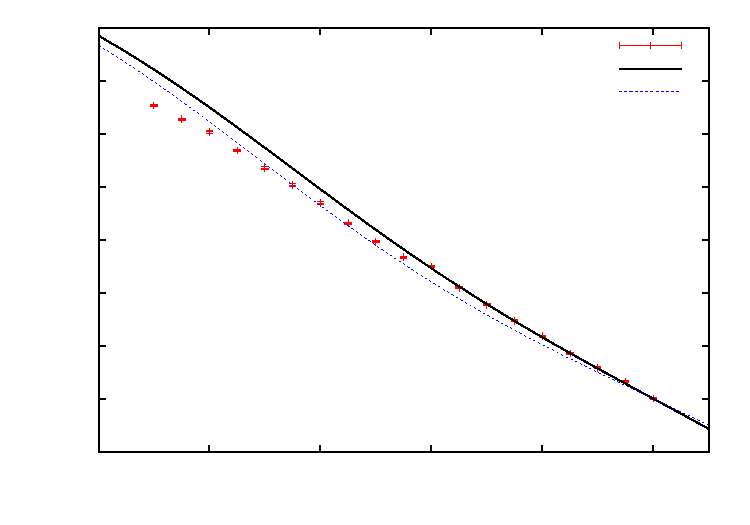
\includegraphics{drehung}}%
    \gplfronttext
  \end{picture}%
\endgroup

	\caption{Drehwinkel $\gamma$ gegen den Einfallswinkel $\alpha$ aufgetragen.}
	\label{fig:drehwinkel}
\end{figure}

Bevor der Strahl auf das Nicol-Prisma trifft, ist er zu gleichen Teilen parallel sowie senkrecht zur Einfallsebene polarisiert.
Da aber beide Polarisationsrichtungen unterschiedlich stark reflektiert werden, ist der ausfallende Strahl um den Winkel $\gamma$ gedreht.
Dieser lässt sich mit
\begin{align}
	\tan(\gamma+45^\circ)=\frac{r_s}{r_p}=-\frac{\cos(\alpha-\beta)}{\cos(\alpha+\beta)}
	\label{eq:theorie}
\end{align}
unter Verwendung von \eqref{eq:r_s} und \eqref{eq:r_p} berechnen.
Einziger Parameter ist dabei das Verhältnis der Brechungsindizes $\frac{n_2}{n_1}$, da $\beta$ über \eqref{eq:snellius} von $\alpha$ abhängt.

Die Drehung der Schwingungsebene konnte nur relativ gemessen werden.
Bei einem Einfallswinkel von $90^\circ$ wird das Licht jedoch nicht gedreht, da in beiden Polarisationsfällen alles reflektiert wird.
Also ist dort $\gamma=0^\circ$.
In Abbildung \ref{fig:drehwinkel} ist der Drehwinkel $\gamma$ gegen den Einfallswinkel $\alpha$ aufgetragen.
Der Messfehler für $\gamma$ beträgt $0.2^\circ$.
Außerdem ist die Theoriekurve nach \eqref{eq:theorie} mit $n=1.51$ eingezeichnet.\\
Zusätzlich kann man den Parameter $n$ noch an die Messwerte anpassen:
Aus dem $\chi^2$-Fit der Theoriekurve  erhält man
\begin{empheq}[box=\shadowbox]{align*}
	n = 1.405 \pm 0.019\,.
\end{empheq}

\subsection{Brechungsindex aus $\gamma=45^\circ$}

\begin{figure}[!htb]
	\centering
	% GNUPLOT: LaTeX picture with Postscript
\begingroup
  \makeatletter
  \providecommand\color[2][]{%
    \GenericError{(gnuplot) \space\space\space\@spaces}{%
      Package color not loaded in conjunction with
      terminal option `colourtext'%
    }{See the gnuplot documentation for explanation.%
    }{Either use 'blacktext' in gnuplot or load the package
      color.sty in LaTeX.}%
    \renewcommand\color[2][]{}%
  }%
  \providecommand\includegraphics[2][]{%
    \GenericError{(gnuplot) \space\space\space\@spaces}{%
      Package graphicx or graphics not loaded%
    }{See the gnuplot documentation for explanation.%
    }{The gnuplot epslatex terminal needs graphicx.sty or graphics.sty.}%
    \renewcommand\includegraphics[2][]{}%
  }%
  \providecommand\rotatebox[2]{#2}%
  \@ifundefined{ifGPcolor}{%
    \newif\ifGPcolor
    \GPcolorfalse
  }{}%
  \@ifundefined{ifGPblacktext}{%
    \newif\ifGPblacktext
    \GPblacktexttrue
  }{}%
  % define a \g@addto@macro without @ in the name:
  \let\gplgaddtomacro\g@addto@macro
  % define empty templates for all commands taking text:
  \gdef\gplbacktext{}%
  \gdef\gplfronttext{}%
  \makeatother
  \ifGPblacktext
    % no textcolor at all
    \def\colorrgb#1{}%
    \def\colorgray#1{}%
  \else
    % gray or color?
    \ifGPcolor
      \def\colorrgb#1{\color[rgb]{#1}}%
      \def\colorgray#1{\color[gray]{#1}}%
      \expandafter\def\csname LTw\endcsname{\color{white}}%
      \expandafter\def\csname LTb\endcsname{\color{black}}%
      \expandafter\def\csname LTa\endcsname{\color{black}}%
      \expandafter\def\csname LT0\endcsname{\color[rgb]{1,0,0}}%
      \expandafter\def\csname LT1\endcsname{\color[rgb]{0,1,0}}%
      \expandafter\def\csname LT2\endcsname{\color[rgb]{0,0,1}}%
      \expandafter\def\csname LT3\endcsname{\color[rgb]{1,0,1}}%
      \expandafter\def\csname LT4\endcsname{\color[rgb]{0,1,1}}%
      \expandafter\def\csname LT5\endcsname{\color[rgb]{1,1,0}}%
      \expandafter\def\csname LT6\endcsname{\color[rgb]{0,0,0}}%
      \expandafter\def\csname LT7\endcsname{\color[rgb]{1,0.3,0}}%
      \expandafter\def\csname LT8\endcsname{\color[rgb]{0.5,0.5,0.5}}%
    \else
      % gray
      \def\colorrgb#1{\color{black}}%
      \def\colorgray#1{\color[gray]{#1}}%
      \expandafter\def\csname LTw\endcsname{\color{white}}%
      \expandafter\def\csname LTb\endcsname{\color{black}}%
      \expandafter\def\csname LTa\endcsname{\color{black}}%
      \expandafter\def\csname LT0\endcsname{\color{black}}%
      \expandafter\def\csname LT1\endcsname{\color{black}}%
      \expandafter\def\csname LT2\endcsname{\color{black}}%
      \expandafter\def\csname LT3\endcsname{\color{black}}%
      \expandafter\def\csname LT4\endcsname{\color{black}}%
      \expandafter\def\csname LT5\endcsname{\color{black}}%
      \expandafter\def\csname LT6\endcsname{\color{black}}%
      \expandafter\def\csname LT7\endcsname{\color{black}}%
      \expandafter\def\csname LT8\endcsname{\color{black}}%
    \fi
  \fi
  \setlength{\unitlength}{0.0500bp}%
  \begin{picture}(7200.00,5040.00)%
    \gplgaddtomacro\gplbacktext{%
      \csname LTb\endcsname%
      \put(814,704){\makebox(0,0)[r]{\strut{} 30}}%
      \put(814,1286){\makebox(0,0)[r]{\strut{} 35}}%
      \put(814,1867){\makebox(0,0)[r]{\strut{} 40}}%
      \put(814,2449){\makebox(0,0)[r]{\strut{} 45}}%
      \put(814,3030){\makebox(0,0)[r]{\strut{} 50}}%
      \put(814,3612){\makebox(0,0)[r]{\strut{} 55}}%
      \put(814,4193){\makebox(0,0)[r]{\strut{} 60}}%
      \put(814,4775){\makebox(0,0)[r]{\strut{} 65}}%
      \put(946,484){\makebox(0,0){\strut{} 46}}%
      \put(1727,484){\makebox(0,0){\strut{} 48}}%
      \put(2508,484){\makebox(0,0){\strut{} 50}}%
      \put(3289,484){\makebox(0,0){\strut{} 52}}%
      \put(4070,484){\makebox(0,0){\strut{} 54}}%
      \put(4851,484){\makebox(0,0){\strut{} 56}}%
      \put(5632,484){\makebox(0,0){\strut{} 58}}%
      \put(6413,484){\makebox(0,0){\strut{} 60}}%
      \put(176,2739){\rotatebox{-270}{\makebox(0,0){\strut{}Drehwinkel $\gamma$ [$^\circ$]}}}%
      \put(3874,154){\makebox(0,0){\strut{}Einfallswinkel $\alpha$ [$^\circ$]}}%
    }%
    \gplgaddtomacro\gplfronttext{%
      \csname LTb\endcsname%
      \put(5816,4602){\makebox(0,0)[r]{\strut{}Messwerte}}%
      \csname LTb\endcsname%
      \put(5816,4382){\makebox(0,0)[r]{\strut{}lineare Regression}}%
      \csname LTb\endcsname%
      \put(5816,4162){\makebox(0,0)[r]{\strut{}Theorie gefittet}}%
      \csname LTb\endcsname%
      \put(5816,3942){\makebox(0,0)[r]{\strut{}Theoriekurve}}%
      \csname LTb\endcsname%
      \put(5816,3722){\makebox(0,0)[r]{\strut{}Brewster-Winkel}}%
    }%
    \gplbacktext
    \put(0,0){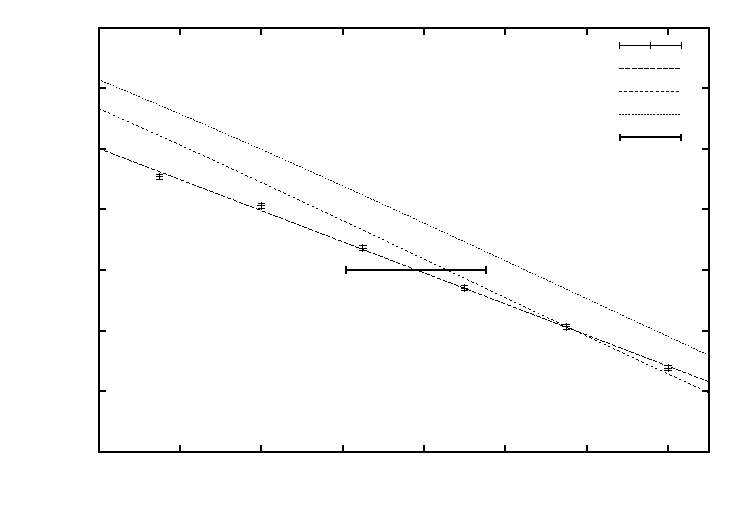
\includegraphics{drehung_zoom}}%
    \gplfronttext
  \end{picture}%
\endgroup

	\caption{$\gamma$ gegen $\alpha$ im Bereich $\gamma=45^\circ$: lineare Regression und Brewster-Winkel}
	\label{fig:drehung_zoom}
\end{figure}

Bei einem Drehwinkel $\gamma=45^\circ$ ist der Einfallswinkel gerade der Brewster-Winkel $\alpha_B$, da dann nach \eqref{eq:theorie} $\cos(\alpha+\beta)=0$ und somit $\alpha+\beta=90^\circ$ gelten muss.
Man kann ihn somit graphisch bestimmen.
Legt man eine Gerade durch die 6 nächsten Werte (vgl. Abb. \ref{fig:drehung_zoom}), erhält man aus der Geradensteigung $m=-1.283 \pm 0.029$ und dem y-Achsenabschnitt 
$b=114.1^\circ \pm 1.6^\circ$ mit
\begin{align}
	\alpha&=\frac{45^\circ-b}{m} \qquad \text{und}\\
	\sigma_\alpha&=\sqrt{\left(\frac{\sigma_b}{m}\right)^2+\left(\frac{45^\circ-b}{m^2}\cdot\sigma_m \right)^2}
\end{align}
den passenden Winkel $\alpha_B=53.8^\circ \pm 1.8^\circ$.
Daraus kann man mit \eqref{eq:brewster} den Brechungsindex des Prismas berechnen.
Der sich dabei ergebende Fehler
\begin{align}
	\sigma_n=\frac{\sigma_\alpha}{\cos^2\alpha}
	\label{eq:brewster_err}	
\end{align}
leitet sich aus der Fehlerfortpflanzung ab.
Man erhält
\begin{empheq}[box=\shadowbox]{align*}
	n = 1.37 \pm 0.10\,.
\end{empheq}


\subsection{Brewster-Winkel}
Zunächst wurden 6 Messwerte für den Brewster-Winkel $\alpha_B$ bzw. den zugehörigen Auslenkwinkel $\Phi_B$ des Schwenkarms aufgenommen.
Dabei ließ sich das Minimum nur schwer finden und die Messwerte schwankten sehr.
Dann wurde der Polaristor um etwa $5^\circ$ gedreht und der Bereich minimaler Intensität war viel schärfer als zuvor.
Es wurden 4 Messwerte aufgenommen.
Wie zuvor auch wechselten sich die Versuchspartner zwischen jedem Messwert ab.
Man kann nun aus allen Werten ein $\Phi_B$ bestimmen oder einzeln für jede Messreihe oder jede Person.
Der Fehler berechnet sich dabei aus der Student-t-Verteilung, da die Anzahl der Messwerte gering ist.
Er halbiert sich für $\alpha_B$.
Mit \eqref{eq:brewster} und \eqref{eq:brewster_err} kann wieder der Brechungsindex berechnet werden.
Die somit berechneten Werte sind in Tabelle \ref{tab:brewster} aufgeführt.
\begin{table}[!htb]
	\centering
	\begin{tabular}{|c|c|c|c|}
		\hline		
		& $\Phi_B$ [$^\circ$] & $\alpha_B$ [$^\circ$] & $n$ \\
		\hline
		Alle Werte & $66.6 \pm 0.6$ & $56.7 \pm 0.3$ & $1.522 \pm 0.018$ \\
		erste Messreihe & $66.4 \pm 0.9$ & $56.8 \pm 0.5$ & $1.53 \pm 0.03$ \\
		zweite Messreihe & $67.0 \pm 0.5$ & $56.50 \pm 0.25$ & $1.511 \pm 0.015$ \\
		\hline
		Michael & $67.3 \pm 0.5$ & $56.35 \pm 0.25$ & $1.502 \pm 0.015$ \\
		Felix & $65.9 \pm 1.0$ & $57.1 \pm 0.5$ & $1.55 \pm 0.03$ \\
		\hline
	\end{tabular}
	\caption{Brewster-Winkel.}
	\label{tab:brewster}
\end{table}

\section{Diskussion}
\label{sec:diskussion}
\subsection{Drehung der Schwingungsebene}
Der Wert für den Brechungsindex $n=1.405 \pm 0.019$ aus dem Fit der Theoriekurve an die Messwerte ist $7\%$ kleiner als der Literaturwert $n=1.51$.
Außerdem  liegt jener nicht im relativ kleinen Fehlerintervall.
Vergleicht man nun in Abbildung \ref{fig:drehwinkel} die Messwerte mit der Theorie ($n=1.51$), stellt man fest, dass diese anfangs, also bei großen $\alpha$, sehr gut passen.
Für kleinere Winkel weichen sie deutlich ab.
Man erkennt einen leichten Sprung bei $\alpha=67.5^\circ$.
Da von $\alpha=90^\circ$ angefangen wurde, zu messen, kann es sein, dass ab der Sprungstelle falsch abgelesen wurde.
Dies verdeutlicht Abbildung \ref{fig:drehung2}.
Dort wird der notierte Winkel um $5^\circ$ nach oben korrigiert, da in diesen Abständen größere Striche auf der Skala des Analysators zur besseren Orientierung vorhanden sind.
So ist der Sprung nun in die andere Richtung ausgeprägt, aber die Werte passen besser zur Theorie.
Allerdings flachen die Messwerte bei kleinem $\alpha$ stärker ab als die theoretische Kurve, sodass diese Erklärung nicht vollständig richtig erscheint.
Um diesen Sachverhalt zu klären, hätte man die Werte nochmal bezüglich der absoluten Position des Analysators kontrollieren müssen.
\begin{figure}[!htb]
	\centering
	% GNUPLOT: LaTeX picture with Postscript
\begingroup
  \makeatletter
  \providecommand\color[2][]{%
    \GenericError{(gnuplot) \space\space\space\@spaces}{%
      Package color not loaded in conjunction with
      terminal option `colourtext'%
    }{See the gnuplot documentation for explanation.%
    }{Either use 'blacktext' in gnuplot or load the package
      color.sty in LaTeX.}%
    \renewcommand\color[2][]{}%
  }%
  \providecommand\includegraphics[2][]{%
    \GenericError{(gnuplot) \space\space\space\@spaces}{%
      Package graphicx or graphics not loaded%
    }{See the gnuplot documentation for explanation.%
    }{The gnuplot epslatex terminal needs graphicx.sty or graphics.sty.}%
    \renewcommand\includegraphics[2][]{}%
  }%
  \providecommand\rotatebox[2]{#2}%
  \@ifundefined{ifGPcolor}{%
    \newif\ifGPcolor
    \GPcolortrue
  }{}%
  \@ifundefined{ifGPblacktext}{%
    \newif\ifGPblacktext
    \GPblacktexttrue
  }{}%
  % define a \g@addto@macro without @ in the name:
  \let\gplgaddtomacro\g@addto@macro
  % define empty templates for all commands taking text:
  \gdef\gplbacktext{}%
  \gdef\gplfronttext{}%
  \makeatother
  \ifGPblacktext
    % no textcolor at all
    \def\colorrgb#1{}%
    \def\colorgray#1{}%
  \else
    % gray or color?
    \ifGPcolor
      \def\colorrgb#1{\color[rgb]{#1}}%
      \def\colorgray#1{\color[gray]{#1}}%
      \expandafter\def\csname LTw\endcsname{\color{white}}%
      \expandafter\def\csname LTb\endcsname{\color{black}}%
      \expandafter\def\csname LTa\endcsname{\color{black}}%
      \expandafter\def\csname LT0\endcsname{\color[rgb]{1,0,0}}%
      \expandafter\def\csname LT1\endcsname{\color[rgb]{0,1,0}}%
      \expandafter\def\csname LT2\endcsname{\color[rgb]{0,0,1}}%
      \expandafter\def\csname LT3\endcsname{\color[rgb]{1,0,1}}%
      \expandafter\def\csname LT4\endcsname{\color[rgb]{0,1,1}}%
      \expandafter\def\csname LT5\endcsname{\color[rgb]{1,1,0}}%
      \expandafter\def\csname LT6\endcsname{\color[rgb]{0,0,0}}%
      \expandafter\def\csname LT7\endcsname{\color[rgb]{1,0.3,0}}%
      \expandafter\def\csname LT8\endcsname{\color[rgb]{0.5,0.5,0.5}}%
    \else
      % gray
      \def\colorrgb#1{\color{black}}%
      \def\colorgray#1{\color[gray]{#1}}%
      \expandafter\def\csname LTw\endcsname{\color{white}}%
      \expandafter\def\csname LTb\endcsname{\color{black}}%
      \expandafter\def\csname LTa\endcsname{\color{black}}%
      \expandafter\def\csname LT0\endcsname{\color{black}}%
      \expandafter\def\csname LT1\endcsname{\color{black}}%
      \expandafter\def\csname LT2\endcsname{\color{black}}%
      \expandafter\def\csname LT3\endcsname{\color{black}}%
      \expandafter\def\csname LT4\endcsname{\color{black}}%
      \expandafter\def\csname LT5\endcsname{\color{black}}%
      \expandafter\def\csname LT6\endcsname{\color{black}}%
      \expandafter\def\csname LT7\endcsname{\color{black}}%
      \expandafter\def\csname LT8\endcsname{\color{black}}%
    \fi
  \fi
  \setlength{\unitlength}{0.0500bp}%
  \begin{picture}(7200.00,5040.00)%
    \gplgaddtomacro\gplbacktext{%
      \csname LTb\endcsname%
      \put(814,704){\makebox(0,0)[r]{\strut{}-10}}%
      \put(814,1213){\makebox(0,0)[r]{\strut{} 0}}%
      \put(814,1722){\makebox(0,0)[r]{\strut{} 10}}%
      \put(814,2231){\makebox(0,0)[r]{\strut{} 20}}%
      \put(814,2740){\makebox(0,0)[r]{\strut{} 30}}%
      \put(814,3248){\makebox(0,0)[r]{\strut{} 40}}%
      \put(814,3757){\makebox(0,0)[r]{\strut{} 50}}%
      \put(814,4266){\makebox(0,0)[r]{\strut{} 60}}%
      \put(814,4775){\makebox(0,0)[r]{\strut{} 70}}%
      \put(946,484){\makebox(0,0){\strut{} 40}}%
      \put(2011,484){\makebox(0,0){\strut{} 50}}%
      \put(3076,484){\makebox(0,0){\strut{} 60}}%
      \put(4141,484){\makebox(0,0){\strut{} 70}}%
      \put(5206,484){\makebox(0,0){\strut{} 80}}%
      \put(6271,484){\makebox(0,0){\strut{} 90}}%
      \put(176,2739){\rotatebox{-270}{\makebox(0,0){\strut{}Drehwinkel $\gamma$ [$^\circ$]}}}%
      \put(3874,154){\makebox(0,0){\strut{}Auftreffwinkel $\alpha$ [$^\circ$]}}%
    }%
    \gplgaddtomacro\gplfronttext{%
      \csname LTb\endcsname%
      \put(5816,4602){\makebox(0,0)[r]{\strut{}Messwerte}}%
      \csname LTb\endcsname%
      \put(5816,4382){\makebox(0,0)[r]{\strut{}Theoriekurve}}%
    }%
    \gplbacktext
    \put(0,0){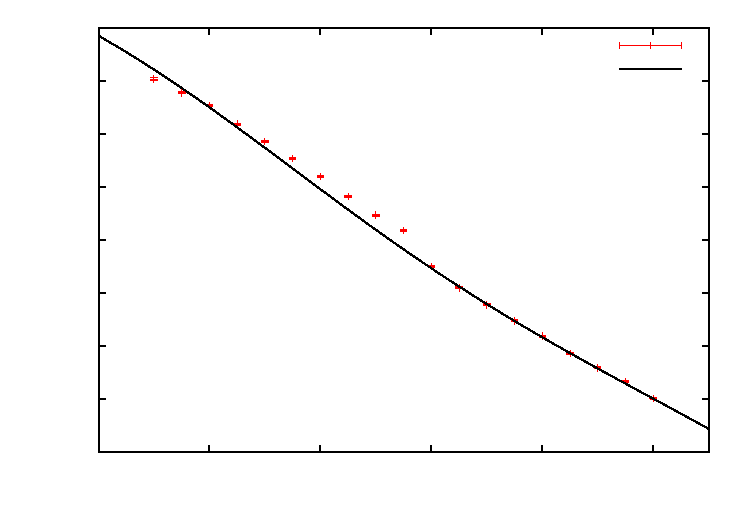
\includegraphics{drehung2}}%
    \gplfronttext
  \end{picture}%
\endgroup

	\caption{$\gamma$ gegen $\alpha$: $\gamma$ um $5^\circ$ nach oben verschoben für $\alpha \leq 67.5^\circ\,$.}
	\label{fig:drehung2}
\end{figure}

Der Wert für den Brechungsindex aus der linearen Regression ist $10\%$ kleiner als der Literaturwert.
Jedoch ist das Fehlerintervall sehr groß und der Maximalwert $n=1.47$ weicht nur $2.7\%$ vom angegebenen Wert ab.
Der Fehlerbalken in Abbildung \ref{fig:drehung_zoom} ist nämlich sehr groß.
Hätte man mehr Messwerte in der Nähe von $\gamma=45^\circ$ aufgenommen, wäre die Gerade genauer bestimmt und so der Fehlerbalken kleiner.
Die Abweichung zur Theoriekurve wird dann aber größer.

Sofern die Messwerte korrekt notiert wurden, deuten sie auf einen sehr viel geringeren Brechungsindex hin.
Der Brechungsindex, der aus dem Brewsterwinkel bestimmt wurde, weicht jedoch nicht so stark vom Literaturwert ab.
Daher muss von einem systematischen Fehler ausgegangen werden.

\subsection{Brewster-Winkel}
Der Brechungsindex, der aus allen Messwerten zum Brewster-Winkel bestimmt wurde, ist minimal größer als der Literaturwert ($< 1\%$) und dieser liegt im Fehlerintervall.
Die Abweichung ist für die zweite Messreihe noch kleiner und sowohl das berechnete Fehlerintervall sowie das angegebene weisen eine große Übereinstimmung auf.
Dies unterstützt die obige Theorie der falschen Polarisatorstellung, da diese Messwerte nach nochmaligem Drehen um etwa $5^\circ$ aufgenommen wurden.
So konnte man das nun dunklere Intensitätsminimum deutlicher erkennen.
Dann ist das ankommende Licht nahezu parallel polarisiert.
Hätte man nun die Messung des Drehwinkels wiederholt, müssten sich bessere Werte ergeben.\\

Auch die anderen Werte in Tabelle \ref{tab:brewster} weisen kaum größere Abweichungen vom Literaturwert ab.
Man erkennt aber trotzdem signifikante Unterschiede in der Genauigkeit der Messung.
So ist der Fehler $\sigma_n=0.03$ bei der ersten Messreihe und den von Felix aufgenommenen Werten etwa doppelt so groß wie die anderen drei Fehlern.
Die Werte für den Brewster-Winkel streuen nämlich sehr, da das Minimum zuerst ziemlich breit war.
Hätte man bei der zweiten Messung öfter gemessen, wäre der Fehler $\sigma_n$ noch deutlich geringer.

\subsection{Falsche Polarisatorstellung}
Die Messung des Brewster-Winkels deutet darauf hin, dass der Polarisator anfangs nicht genau um $45^\circ$ gedreht war.
Dies hätte zur Folge, dass das Licht nicht zur Hälfte parallel polarisiert und zur anderen senkrecht polarisiert ist, wenn es auf das Prisma fällt.
Somit wäre die Formel \eqref{eq:theorie} falsch.
Eine mögliche Ursache für die Abweichung vom korrekten Polarisationswinkel könnte das Verwenden von zwei Prismen sein.
So wurde das kleinere Nicol-Prisma zur Justage verwendet und das andere im Analysator zur Messung.
Dies erhöht die Fehlerquellen, da das Kleine nicht richtig ausgerichtet sein kann und beide aufgrund der Bauweise etwas unterschiedliche optische Eigenschaften haben könnten.

Ist das Licht im Winkel $\delta$ zur optischen Achse polarisiert, muss Formel \eqref{eq:theorie} korrigiert werden.
So ist das Verhältnis zwischen senkrecht und parallel polarisiertem Licht vor dem Prisma genau $\tan\delta$.
Damit ergibt sich

\begin{align}
	\tan(\gamma+\delta)=\tan(\delta)\cdot\frac{r_s}{r_p}=-\tan(\delta)\cdot\frac{\cos(\alpha-\beta)}{\cos(\alpha+\beta)}\,,
	\label{eq:theorie_verbessert}
\end{align}
wobei wieder \eqref{eq:snellius} gilt.

Fittet man den Parameter $\delta$ dieser Kurve an die Messwerte bei festem $n=1.51$ wie in Abbildung \ref{fig:drehung_disk} ergibt sich für die Polarisatorstellung $\delta=48.68^\circ \pm 0.19^\circ$.
Dies sind also etwa $3.7^\circ$ mehr als die gewünschten $45^\circ$ und deckt sich mit der Drehung um etwa 5 weitere Grad zur besseren Messung des Brewster-Winkels.
Am Polarisator sind nämlich nur Markierungen von vorigen Versuchsdurchführungen, die in keinem festen Abstand zueinander sind.
So konnte der zusätzlich Drehwinkel nur grob abgeschätzt werden.
Nun sind die Messwerte sehr viel näher an der Theoriekurve und die obige Annahme wird bestätigt.
Der zuvor diskutierte Ablesefehler ist nicht zu erkennen.
Lediglich der Messwert bei $\alpha=70^\circ$ ist ein wenig zu groß.\\

Um den Fehler der falschen Polarisatorstellung zu vermeiden, hätte man also erst den Brewster-Winkel und dann die Drehung der Schwingungsebene messen sollen.
Kennt man die Polarisatorstellung $\delta$ nämlich nicht, ist die  Formel \eqref{eq:theorie_verbessert} von zwei Parametern abhängig: $n$ und $\delta$.
Ein $\chi^2$-Fit mit beiden ist nicht sinnvoll, da sich die Effekte der beiden Parameter in gewissen Grenzen aufheben.
Deshalb erhält man damit keinen vernünftigen Wert für den Brechungsindex $n$.

\begin{figure}[!htb]
	\centering
	% GNUPLOT: LaTeX picture with Postscript
\begingroup
  \makeatletter
  \providecommand\color[2][]{%
    \GenericError{(gnuplot) \space\space\space\@spaces}{%
      Package color not loaded in conjunction with
      terminal option `colourtext'%
    }{See the gnuplot documentation for explanation.%
    }{Either use 'blacktext' in gnuplot or load the package
      color.sty in LaTeX.}%
    \renewcommand\color[2][]{}%
  }%
  \providecommand\includegraphics[2][]{%
    \GenericError{(gnuplot) \space\space\space\@spaces}{%
      Package graphicx or graphics not loaded%
    }{See the gnuplot documentation for explanation.%
    }{The gnuplot epslatex terminal needs graphicx.sty or graphics.sty.}%
    \renewcommand\includegraphics[2][]{}%
  }%
  \providecommand\rotatebox[2]{#2}%
  \@ifundefined{ifGPcolor}{%
    \newif\ifGPcolor
    \GPcolortrue
  }{}%
  \@ifundefined{ifGPblacktext}{%
    \newif\ifGPblacktext
    \GPblacktexttrue
  }{}%
  % define a \g@addto@macro without @ in the name:
  \let\gplgaddtomacro\g@addto@macro
  % define empty templates for all commands taking text:
  \gdef\gplbacktext{}%
  \gdef\gplfronttext{}%
  \makeatother
  \ifGPblacktext
    % no textcolor at all
    \def\colorrgb#1{}%
    \def\colorgray#1{}%
  \else
    % gray or color?
    \ifGPcolor
      \def\colorrgb#1{\color[rgb]{#1}}%
      \def\colorgray#1{\color[gray]{#1}}%
      \expandafter\def\csname LTw\endcsname{\color{white}}%
      \expandafter\def\csname LTb\endcsname{\color{black}}%
      \expandafter\def\csname LTa\endcsname{\color{black}}%
      \expandafter\def\csname LT0\endcsname{\color[rgb]{1,0,0}}%
      \expandafter\def\csname LT1\endcsname{\color[rgb]{0,1,0}}%
      \expandafter\def\csname LT2\endcsname{\color[rgb]{0,0,1}}%
      \expandafter\def\csname LT3\endcsname{\color[rgb]{1,0,1}}%
      \expandafter\def\csname LT4\endcsname{\color[rgb]{0,1,1}}%
      \expandafter\def\csname LT5\endcsname{\color[rgb]{1,1,0}}%
      \expandafter\def\csname LT6\endcsname{\color[rgb]{0,0,0}}%
      \expandafter\def\csname LT7\endcsname{\color[rgb]{1,0.3,0}}%
      \expandafter\def\csname LT8\endcsname{\color[rgb]{0.5,0.5,0.5}}%
    \else
      % gray
      \def\colorrgb#1{\color{black}}%
      \def\colorgray#1{\color[gray]{#1}}%
      \expandafter\def\csname LTw\endcsname{\color{white}}%
      \expandafter\def\csname LTb\endcsname{\color{black}}%
      \expandafter\def\csname LTa\endcsname{\color{black}}%
      \expandafter\def\csname LT0\endcsname{\color{black}}%
      \expandafter\def\csname LT1\endcsname{\color{black}}%
      \expandafter\def\csname LT2\endcsname{\color{black}}%
      \expandafter\def\csname LT3\endcsname{\color{black}}%
      \expandafter\def\csname LT4\endcsname{\color{black}}%
      \expandafter\def\csname LT5\endcsname{\color{black}}%
      \expandafter\def\csname LT6\endcsname{\color{black}}%
      \expandafter\def\csname LT7\endcsname{\color{black}}%
      \expandafter\def\csname LT8\endcsname{\color{black}}%
    \fi
  \fi
  \setlength{\unitlength}{0.0500bp}%
  \begin{picture}(7200.00,5040.00)%
    \gplgaddtomacro\gplbacktext{%
      \csname LTb\endcsname%
      \put(814,704){\makebox(0,0)[r]{\strut{}-10}}%
      \put(814,1213){\makebox(0,0)[r]{\strut{} 0}}%
      \put(814,1722){\makebox(0,0)[r]{\strut{} 10}}%
      \put(814,2231){\makebox(0,0)[r]{\strut{} 20}}%
      \put(814,2740){\makebox(0,0)[r]{\strut{} 30}}%
      \put(814,3248){\makebox(0,0)[r]{\strut{} 40}}%
      \put(814,3757){\makebox(0,0)[r]{\strut{} 50}}%
      \put(814,4266){\makebox(0,0)[r]{\strut{} 60}}%
      \put(814,4775){\makebox(0,0)[r]{\strut{} 70}}%
      \put(946,484){\makebox(0,0){\strut{} 40}}%
      \put(2011,484){\makebox(0,0){\strut{} 50}}%
      \put(3076,484){\makebox(0,0){\strut{} 60}}%
      \put(4141,484){\makebox(0,0){\strut{} 70}}%
      \put(5206,484){\makebox(0,0){\strut{} 80}}%
      \put(6271,484){\makebox(0,0){\strut{} 90}}%
      \put(176,2739){\rotatebox{-270}{\makebox(0,0){\strut{}Drehwinkel $\gamma$ [$^\circ$]}}}%
      \put(3874,154){\makebox(0,0){\strut{}Einfallswinkel $\alpha$ [$^\circ$]}}%
    }%
    \gplgaddtomacro\gplfronttext{%
      \csname LTb\endcsname%
      \put(5816,4602){\makebox(0,0)[r]{\strut{}Messwerte}}%
      \csname LTb\endcsname%
      \put(5816,4382){\makebox(0,0)[r]{\strut{}Theoriekurve}}%
    }%
    \gplbacktext
    \put(0,0){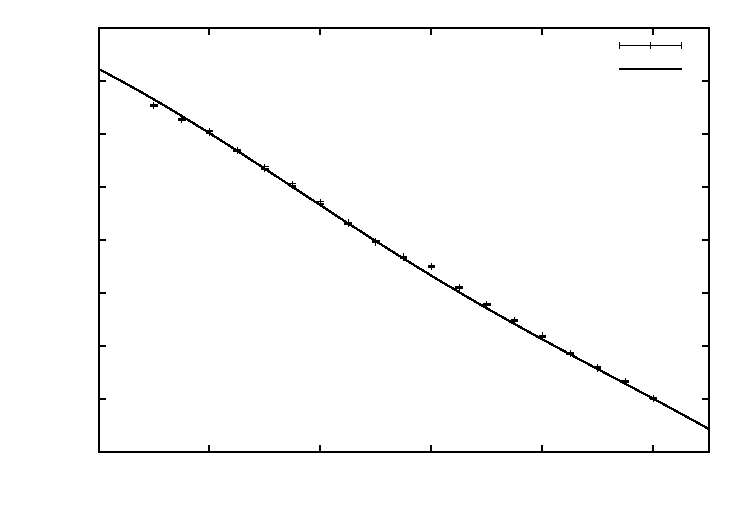
\includegraphics{drehung_disk}}%
    \gplfronttext
  \end{picture}%
\endgroup

	\caption{$\gamma$ gegen $\alpha$: verbesserte Theoriekurve nach \eqref{eq:theorie_verbessert} mit $\delta=48.68^\circ$.}
	\label{fig:drehung_disk}
\end{figure}


\bibliography{literatur}
\bibliographystyle{babalpha}

\end{document}
